%version 1.00,	date 12/05/2016	auteur(s) Pierre Porche
\speaker{\Julie}

\begin{frame}
\frametitle{Aide à l'attribution des interventions}
	\begin{minipage}[c]{.40\linewidth}
      \begin{figure}[r]
		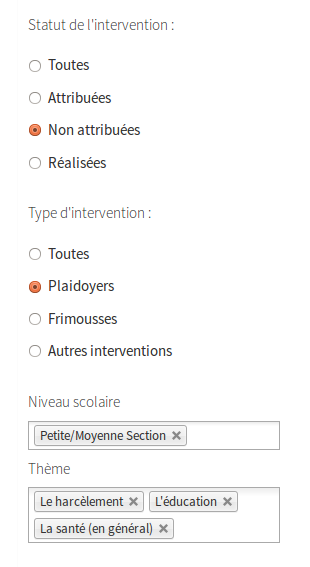
\includegraphics[scale=0.35]{images/filtreListeIntervention.png}
		%\caption{Imprim-écran des possibilités de tris}
	  \end{figure}
   \end{minipage} \hfill
   \begin{minipage}[c]{.52\linewidth}
      \begin{block}{Les filtres}
		\begin{itemize}
			\item requêtes sur la base de données
			\item notion de \texttt{Repository}
		\end{itemize}
	  \end{block}
	  \begin{block}{Rôle des \texttt{Repository}}
		Un repository permet de centraliser tout ce qui touche à la récupération des entités.
		\begin{itemize}
		\item \texttt{class} PHP
		\item \texttt{extends EntityRepository}
		\end{itemize}
	  \end{block}
   \end{minipage} \hfill
\end{frame}

\begin{frame}
\frametitle{La sélection en base de données}
	\begin{block}{Les méthodes de récupération des entités}
		\begin{itemize}
			\item méthodes de récupération de base : \\
			 \texttt{find, findAll, findBy, findOneBy, findByX, findOneByX}
			\item méthodes de récupération personnelle : \\
			\begin{itemize}
			\item \texttt{DQL (Doctrine Query Language)} : \texttt{SQL adapté à la vision objets}
			\item \texttt{Query Builder}: construction de la requête étape par étape
			\end{itemize}			
		\end{itemize}
	  \end{block}
\end{frame}

\begin{frame}
\frametitle{\texttt{Query Builder}}
	\textbf{But :} récupérer les interventions attribuées au bénévole courant. \\
	\vskip 0.5cm
	\begin{block}{Requête SQL :}	
	\texttt{ 
	\noindent $\backslash$set idUtilisateurCourant 10 \\ 	
	SELECT * FROM intervention i, benevole b \\
	\setlength{\parindent}{1cm}	WHERE i.id\_benevole = b.id\\
	\setlength{\parindent}{1cm}	AND WHERE b.id = :idUtilisateurCourant;}
	\end{block}
	\begin{block}{Requête Query Builer :}
	\noindent \texttt{\$qb = \$this->createQueryBuilder('i'); \\
	\noindent \$qb \\
	\setlength{\parindent}{1cm} ->where('i.benevole = :user') \\
    \setlength{\parindent}{1cm} ->setParameter('user', \$user);}
	\end{block}
\end{frame}

\begin{frame}
\frametitle{Attribution/réalisation d'une intervention}
      \begin{figure}[r]
		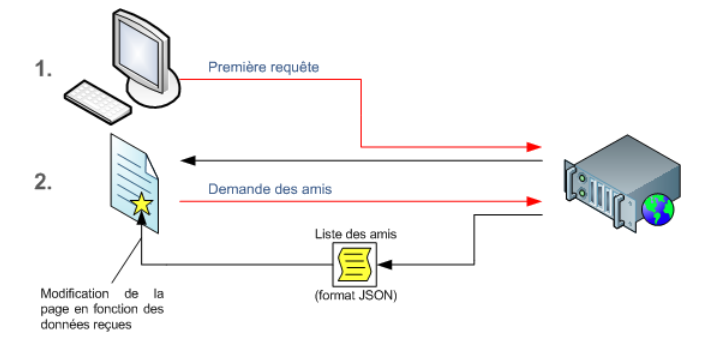
\includegraphics[scale=0.35]{images/ajax.png}
		%\caption{Imprim-écran des possibilités de tris}
	  \end{figure}
      \begin{block}{AJAX (Asynchronous JavaScript And XML)}
		Ajax est un concept de programmation Web dont le but est de faire communiquer une page Web avec un serveur Web recharger de la page.
	  \end{block}
\end{frame}
